%%%%%%%%%%%%%%%%%%%%%%%%%%%%%%%%%%%%%%%%%%%%%%%%%%%%%%%%%%%%%%%%%%%%%%%%%%%%%%%%%%%%%%%%%%%%%%
%%%%%%%%%%%%%%%%%%%%%%%%%%%%%%%%%%%%%%%%%%%%%%%%%%%%%%%%%%%%%%%%%%%%%%%%%%%%%%%%%%%%%%%%%%%%%%
%%%%%%%%%%% systemOverview
%%%%%%%%%%%%%%%%%%%%%%%%%%%%%%%%%%%%%%%%%%%%%%%%%%%%%%%%%%%%%%%%%%%%%%%%%%%%%%%%%%%%%%%%%%%%%%
%%%%%%%%%%%%%%%%%%%%%%%%%%%%%%%%%%%%%%%%%%%%%%%%%%%%%%%%%%%%%%%%%%%%%%%%%%%%%%%%%%%%%%%%%%%%%%


% \cleardoublepage
\chapter{System Overview}
\label{sec:systemOverview}

\section{Overview}
This thesis gives and overview of the the GPU implementation and performance of data aided equalizes.
but the focus of this thesis is on the computation and application of the equalizers.
Before data-aided equalizers can be computed and applied: the preambles must found, the signal packetized, the signal "de-rotated" then the channel and noise variance estimated from the de-rotated signal.
The equalizers are then computed and applied using the de-rotated signal and the estimated channel and noise variance.
After the equalizers have been applied a OQPSK detector is applied to the output of each equalizer.
A simple block Diagram is shown in Figure \ref{fig:simpleBlockDiagram}.
\begin{figure}
	\centering\includegraphics[width=6in]{figures/systemOverview/blockDiagram.pdf}
	\caption{This a simple block diagram of what the GPU does.}
	\label{fig:simpleBlockDiagram}
\end{figure}

This chapter will proceed as follows, 
section \ref{sec:preamble_detection} will explain the GPU implementation of the finding the preambles and packetizing the received signal,
section \ref{sec:frequency_offset_estimation_and_compensation} will explain the GPU implementation of estimating the frequency offset and de-rotating the signal,
section \ref{sec:channel_estimation} will explain the GPU implementation of estimating the channel,
section \ref{sec:noise_variance_estimation} will explain the GPU implementation of estimating the noise variance,
section \ref{sec:oqpsk_detector} will explain the GPU implementation of the OQPSK detector.
The explanation of the GPU implantation of the equalizers will be explained in much detail in Chapter \ref{sec:eq_eq}.





















\subsection{Preamble Detection}
\label{sec:preamble_detection}
The received samples in the project has the iNET packet structure shown in Figure \ref{fig:packet}.
The iNET packet consists of a preamble and ASM periodically inserted into the data stream.
In this project the iNET preamble and ASM bits are inserted every 6144 data bits.
The received signal is sampled at 2 samples/bit, making a iNET packet $12672$ samples long or $\Lpkt$.
The iNET preamble comprises eight repetitions of the 16-bit sequence $\text{CD98}_\text{hex}$ and the ASM field is
\begin{equation}
034776C72728950B0_\text{hex}
\end{equation}
The iNET packet and received sample structure is shown in Figure\ref{fig:packet}.
\begin{figure}
	\centering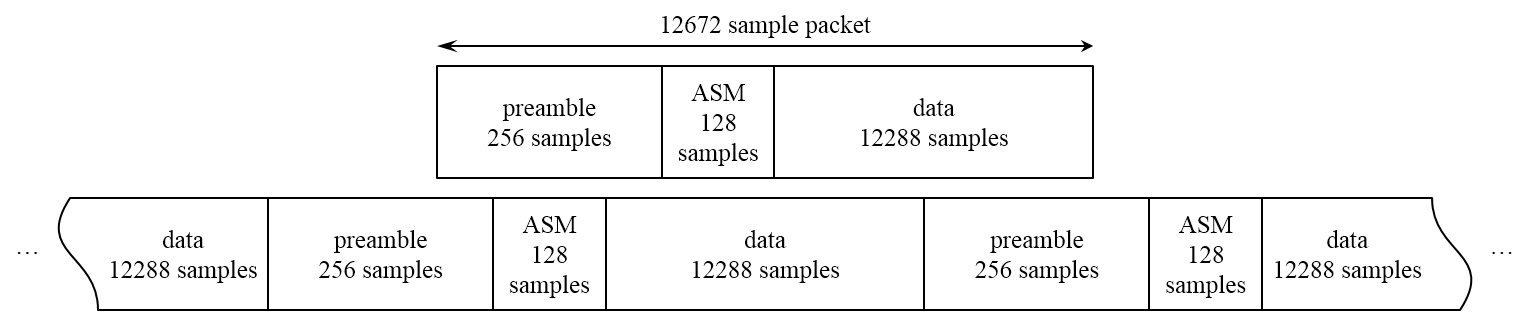
\includegraphics[width=\textwidth]{figures/gpu/packet.png}
	\caption{The iNET packet structure.}
	\label{fig:packet}
\end{figure}

To compute data-aided preamble assisted equalizers, preambles in the received signal are found to estimate various parameters.
The goal of the preamble detection step is to "packetize" the received samples into vectors with the packet structure shown in Figure \ref{fig:packet}.
Before the received samples can be packetized, the preambles are found using a preamble detector to locate the iNET preambles. 
The preamble detector used in this project is the algorithm explained in \cite{preamble_detector}.
Peaks in the preamble detector output indicate the start a preamble.
Using the index of these peaks the received samples can be packetized.

When the received samples are packetized, $\rpkt$ shown in Figure \ref{fig:simpleBlockDiagram} contains one packet worth of samples with the packet structure shown in Figure \ref{fig:packet}.
The received samples are packetized by running the preamble detector and searching the output for peaks.
Starting at each peak index a vector $\rpkt$ is built for each packet.

\subsubsection{The Preamble Detector}
To find the preambles in the batch, the preamble detector computes the sample correlation function between the received samples and a stored local copy of the known samples of the iNET preamble. 
A peak in the correlation function indicates the start of a preamble in the received samples. 
The preamble detector output peaks are found be searching for local peaks that are about $\Lpkt$ samples apart.

The preamble detector detailed in \cite{preamble_detector} is a highly optimized correlator used to compute to how a signal correlates with the iNET preamble eight repetitions of the 16-bit sequence $\text{CD98}_\text{hex}$.
The preamble detector outer summation is
\begin{equation}
	L(u) = \sum_{m=0}^{7}
		\left[ I^2(n,m) + Q^2(n,m) \right]
	\label{eq:gpu-L-4}
\end{equation}
where the inner summations are
\begin{multline}
	I(n,m) \approx \sum_{\ell\in\mathcal{L}_1}r_R(\ell+32m+n)
			- \sum_{\ell\in\mathcal{L}_2}r_R(\ell+32m+n)
			+ \sum_{\ell\in\mathcal{L}_3}r_I(\ell+32m+n)
			- \sum_{\ell\in\mathcal{L}_4}r_I(\ell+32m+n)
			\\
			+ 0.7071 \left[
				\sum_{\ell\in\mathcal{L}_5}r_R(\ell+32m+n)
				- \sum_{\ell\in\mathcal{L}_6}r_R(\ell+32m+n)
			\right. \\
			\left.
				+ \sum_{\ell\in\mathcal{L}_7}r_I(\ell+32m+n)
				- \sum_{\ell\in\mathcal{L}_8}r_I(\ell+32m+n)
			\right],
	\label{eq:gpu-L-pedone-geoghegan-2}
\end{multline}
and
\begin{multline}
	Q(n,m) \approx \sum_{\ell\in\mathcal{L}_1}r_I(\ell+32m+n)
			- \sum_{\ell\in\mathcal{L}_2}r_I(\ell+32m+n)
			\\
			- \sum_{\ell\in\mathcal{L}_3}r_R(\ell+32m+n)
			+ \sum_{\ell\in\mathcal{L}_4}r_R(\ell+32m+n)
			\\
			+ 0.7071 \left[
				\sum_{\ell\in\mathcal{L}_5}r_I(\ell+32m+n)
				- \sum_{\ell\in\mathcal{L}_6}r_I(\ell+32m+n)
			\right. \\
			\left.
				- \sum_{\ell\in\mathcal{L}_7}r_R(\ell+32m+n)
				+ \sum_{\ell\in\mathcal{L}_8}r_R(\ell+32m+n)
			\right]
		\label{eq:gpu-L-pedone-geoghegan-3}
\end{multline}
with
\begin{equation}
	\begin{split}
	\mathcal{L}_1 &= \{ 0, 8, 16, 24 \}\\
	\mathcal{L}_2 &= \{ 4, 20 \}\\
	\mathcal{L}_3 &= \{ 2, 10, 14, 22 \}\\
	\mathcal{L}_4 &= \{ 6, 18, 26, 30 \}\\
	\mathcal{L}_5 &= \{ 1, 7,  9, 15, 17, 23, 25, 31 \}\\
	\mathcal{L}_6 &= \{ 3, 5, 11, 12, 13, 19, 21, 27, 28, 29 \}\\
	\mathcal{L}_7 &= \{ 1, 3,  9, 11, 12, 13, 15, 21, 23 \}\\
	\mathcal{L}_8 &= \{ 5, 7, 17, 19, 25, 27, 28, 29, 31 \}.
\end{split}
\label{eq:gpu-L-pedone-geoghegan-4}
\end{equation}

The preamble detector in Equations \eqref{eq:gpu-L-4}-\eqref{eq:gpu-L-pedone-geoghegan-4} are easily implemented into a GPU.
Two GPU kernels compute the preamble detector output .
The first kernel computes the inner summations and the second computes the outer summation.
In both kernels, one thread to received signal is launched.

\subsubsection{Searching for the Starting Indices}
Equipped with the preamble detector output, $L(u)$ is searched for local maximums or peaks to find the starting index for each preamble.
Figure \ref{fig:L_2_packets} shows $2\times L_{pkt} $ samples of $L(u)$.
The local peaks of $L(u)$ in indicate a preamble starts at the peak's sample index.
A packet starts at sample index $7040$ and $19712$.
The difference between these sample indices is $\Lpkt$, this difference agrees with the packet length shown in Figure \ref{fig:packet}.
\begin{figure}
	\centering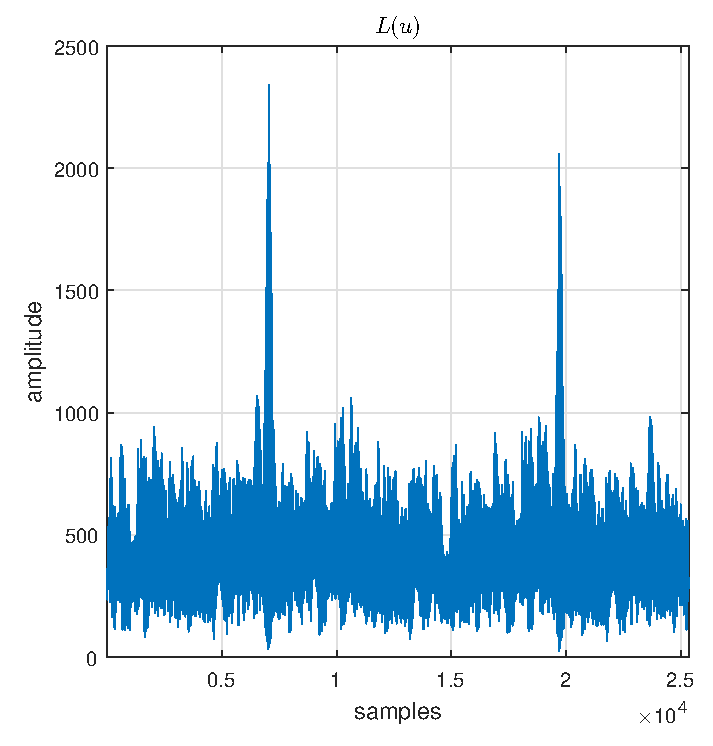
\includegraphics[width=5in]{figures/gpu/L_2_packets.eps}
	\caption{The output of the Preamble Detector $L(u)$.}
	\label{fig:L_2_packets}
\end{figure}

Because of the repetitive structure of the preamble, the preamble detector output $L(u)$ has some unique properties.
The Figures in \ref{fig:L_corr_creepy} show the correlation function around a correlation peak.
The correlation functions have peaks every 32 samples because the repeated $\text{CD98}_\text{hex}$ pattern.

With ideal received samples, 512 samples of $L(u)$ looks like Figure \ref{fig:L_corr_creepy}(a).
The structure of the correlation peaks still occur when the signal to noise ratio is low, as shown in Figure \ref{fig:L_corr_creepy}(b).
But when the signal to noise ratio is low and major multipath distortion happen, the correlation peaks look like Figures \ref{fig:L_corr_creepy}(c) and (d).
The structure of the correlation peaks can cause a local maximum 32 samples off of the start of a preamble.

The preamble detector output is searched for the peak indices using $\Lpkt$ sample windows to ensure only one correlation peak is searched.
The peak indices are checked to ensure each peak index is $\Lpkt$ away from adjacent peak indices.
One GPU kernel searches $L(u)$ for peaks to find the the starting index of each packet.
A thread per $\Lpkt$ received samples is launched to search a window for a local maximum or correlation peak.

In the worst case scenario, a simple algorithm might find an incorrect preamble index by searching a poorly placed search window.
A poorly placed window might search the large side correlation peaks from Figure \ref{fig:L_corr_creepy}(a) and the small main correlation peaks from Figures \ref{fig:L_corr_creepy}(c) or (d).
Because the first three side peaks in Figure \ref{fig:L_corr_creepy}(a) are much taller than the main peak in Figures \ref{fig:L_corr_creepy}(c) and (d), an incorrect preamble starting indices will result if search windows are not defined safely.
\begin{figure}
	\begin{center}
		\begin{tabular}{cc}
			\begin{minipage}[c]{3in}
				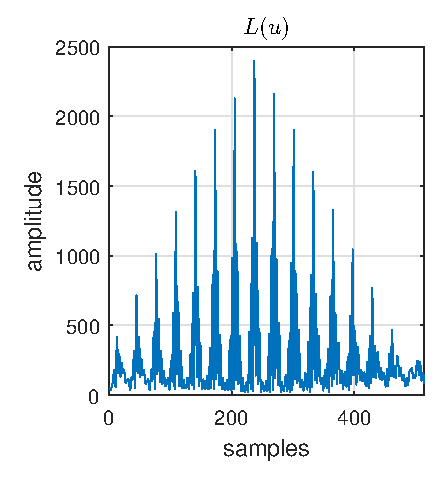
\includegraphics[width=3in]{figures/gpu/L_corr_8_clean.eps}
			\end{minipage} 
			&  
			\begin{minipage}[c]{3in}
				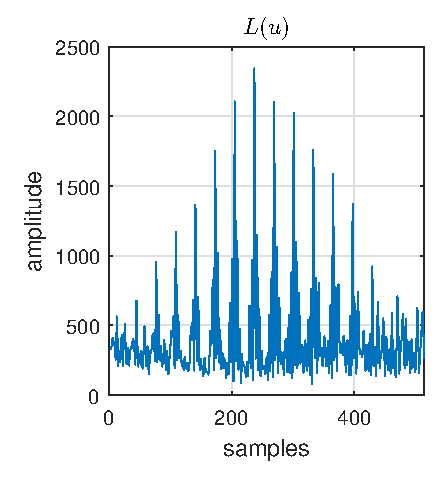
\includegraphics[width=3in]{figures/gpu/L_corr_8_noise.eps}
			\end{minipage} \\[12pt]
			
			\quad\quad\quad\quad(a)
			&
			\quad\quad\quad\quad(b) \\[12pt]
			
			\begin{minipage}[c]{3in}
				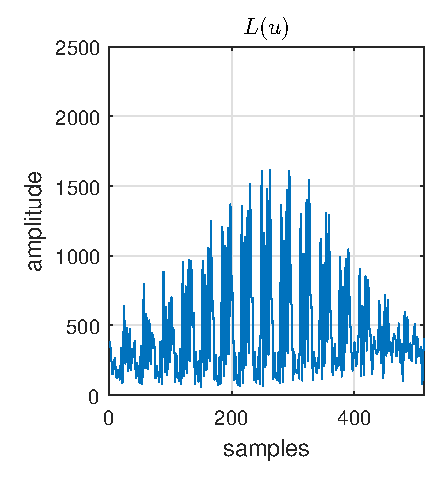
\includegraphics[width=3in]{figures/gpu/L_corr_17_creepy.eps}
			\end{minipage} 
			&  
			\begin{minipage}[c]{3in}
				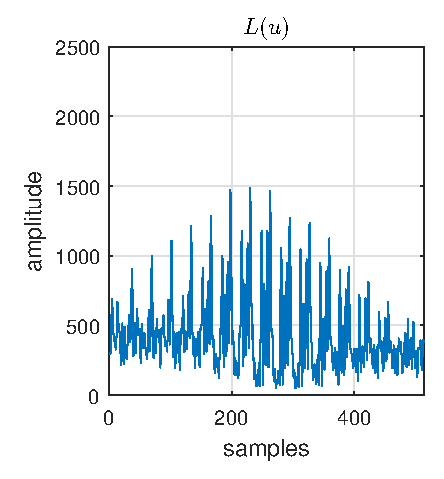
\includegraphics[width=3in]{figures/gpu/L_corr_18_creepy.eps}
			\end{minipage} \\[12pt]
			
			\quad\quad\quad\quad(c)
			&
			\quad\quad\quad\quad(d)
			
		\end{tabular}
	\end{center}
	\caption{Detailed view of $L(u)$. 
			(a): correlation peaks of a distortion free and noiseless signal; 
			(b): correlation peaks of a distortion free but noisy signal with $E_b/N_0 = 0$dB; 
			(c): correlation peaks of a distorted and noisy signal with $E_b/N_0 = 0$dB;
			(d): correlation peaks of a distorted and noisy signal with $E_b/N_0 = 0$dB}
	\label{fig:L_corr_creepy}
\end{figure}

To prevent searching multiple sets of preamble correlation peaks, search windows should only search the correlation peak of one preamble.
Windows are safely defined by centering them on an initial search is done on $2\Lpkt$ received samples to find the estimated index of the first preamble $\hat{i}_0$.
Figure \ref{fig:L_windows} shows an example of safe search windows centered on expected preamble starting locations.
\begin{figure}
	\centering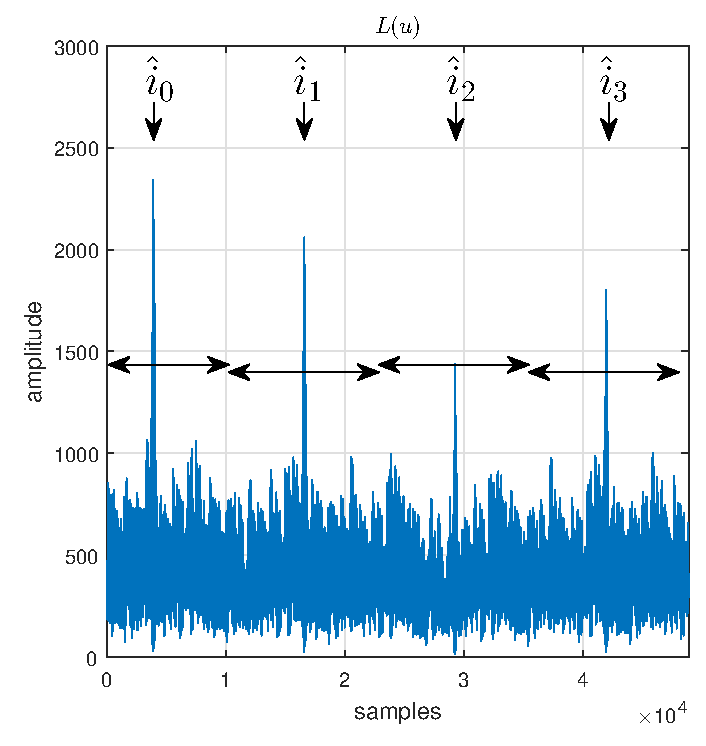
\includegraphics[width=5in]{figures/gpu/L_windows.eps}
	\caption{Safe search windows defined to search only one preamble correlation peak.}
	\label{fig:L_windows}
\end{figure}
The vector
\begin{align}
\hat{\mathbf{i}}
=     
\begin{bmatrix}
\hat{i}_0 	\\
\hat{i}_1	\\
\vdots		\\
\hat{i}_{3103}	\\
\hat{i}_{3104}  		
\end{bmatrix}
\label{eq:preamble_det_i_hat}
\end{align}
is built by the GPU search kernel.
The vector $\hat{\mathbf{i}}$ is a vector of rough estimates of where the preambles should be located.
The windows in the GPU search kernel are centered on elements of $\hat{\mathbf{i}}$ as shown in Figure \ref{fig:L_windows}.
Adjustments are made to the peak index vector $\hat{\mathbf{i}}$ is checked for $\Lpkt$ spacing.

\clearpage
\subsubsection{Packetizing the Samples}
Finally, with the best estimate of the preamble starting locations, the received samples can be packetized.
Using $\hat{\mathbf{i}}$, the GPU launches one thread per received sample to packetize $r(n)$ into $\mathbf{r}_\text{pkt}$ as shown in Figure \ref{fig:packetized}. 
The structure of $\mathbf{r}_\text{pkt}$ majorly simplifies indexing and removes the need for $\hat{\mathbf{i}}$.
\begin{equation}
\mathbf{r}_\text{pkt} = 
\begin{bmatrix}
r(\hat{i}_0) 			\\
r(\hat{i}_0+1) 		\\
\vdots			\\
r(\hat{i}_0+12670)\\
r(\hat{i}_0+12671)\\
r(\hat{i}_1) 			\\
r(\hat{i}_1+1) 		\\
\vdots			\\
r(\hat{i}_{3103}+12670)\\
r(\hat{i}_{3103}+12671)\\
\end{bmatrix}
\end{equation}
%\begin{figure}
%	\centering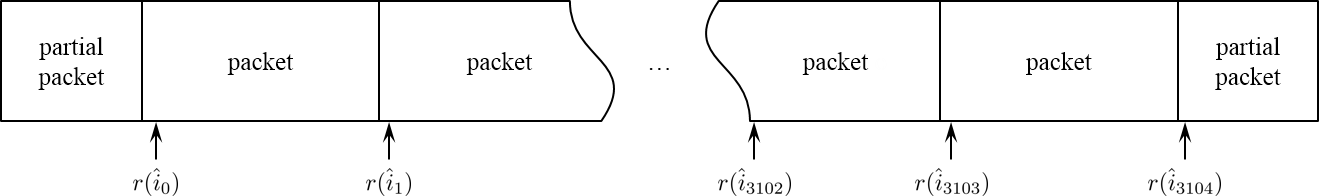
\includegraphics[width=\textwidth/10*9]{figures/gpu/packets_in_batch.png}
%	\caption{The starting sample index for each packet in the batch.}
%	\label{fig:packets_in_batch}
%\end{figure}
\begin{figure}
	\centering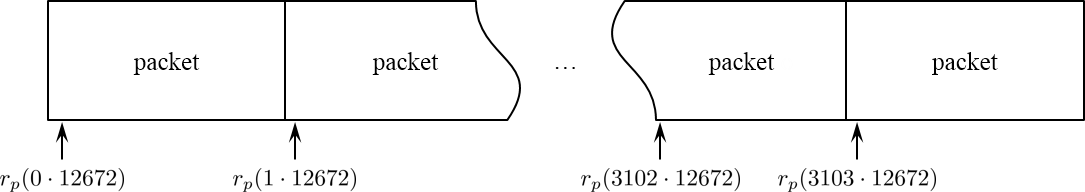
\includegraphics[width=\textwidth/10*9]{figures/gpu/packetized.png}
	\caption{The packetized structure of the received signals after the frame synchronization step.}
	\label{fig:packetized}
\end{figure}

\subsection{Frequency Offset Estimation and Compensation}
\label{sec:frequency_offset_estimation_and_compensation}
With the vector $\mathbf{r}_\text{pkt}$ built, estimators can now easily use the preamble to estimate various parameters.

\subsection{Channel Estimation}
\label{sec:channel_estimation}

\subsection{Noise Variance Estimation}
\label{sec:noise_variance_estimation}

\subsection{OQPSK Detector}
\label{sec:oqpsk_detector}

%\section{System Pictures}
%
%\section{Block Diagram}
%
%\section{Equations}
%
%\subsection{Estimators}
%\subsubsection{Preamble Detector}
%
%\subsection{Equalizers}
%
%\subsection{Decisions}
